\chapter{Problem Statement and Hardware Selecting} \label{ch:hardware}
We want to develop a low-cost, easy to install doorway human counter device for room occupancy estimation. The main component of the device is a low-resolution thermal camera to guarantee privacy protection as well as detection of static human being. Relative counting is done by tracking the human object passing through the doorway and determine whether it is an entering or exiting event. Final occupancy estimation of a room could be obtained by accumulating all relative counts of a device, or several devices, in case of a room with multiple entrances.

The captured image frames should be sent to a microprocessor where the detector and tracker algorithms are implemented. When a frame sequence terminates and the relative count is obtained, this count value should be transferred to a data centralization platform for further processing and long term storage. The data transfer should be wireless to ensure easy installation of the device. We want to keep the device design as simple as possible with minimal components. A Wifi-MCU (micro-controller unit) would be an ideal choice because no other radio components are needed.
\section{Infrared Camera}
For the IR-camera we have considered two candidates: the MLX90640 from melexis and the Amg8833 Grideye from Panasonic. The main attributes of both cameras are listed in \autoref{tab:ircameras}. Among all the technical features, a sufficiently high frame rate is essential so that the whole traversing event could be captured. When installed at a height of 2 meters, both cameras cover about 2.3m along the moving direction. If we subtract the border where a human is partially seen, the valid length left for tracking is merely about 1.7m. Assuming human walking speed is $1.4m/s$, a normal traverse event will last about 1 second. And at least 3 frames should be captured for a simple single-human event. More frames are required for a complex scenario. Overall a minimal frame rate of 8Hz should be reached.

The MLX90640 outperforms AMG8833 in accuracy and resolution. Though we are aware that a better camera may simplify the algorithm design drastically, the AMG8833 is chosen because of its low cost.
\begin{table}[]
\caption{Comparison of the MLX90640 and AMG8833}\label{tab:ircameras}
\centering
\begin{tabular}{lll}
                                      & MLX90640                                      & AMG8833                  \\ \hline
\multicolumn{1}{l|}{resolution}       & \multicolumn{1}{l|}{32$\times$24}             & 8$\times$8               \\
\multicolumn{1}{l|}{frame rate}       & \multicolumn{1}{l|}{0.5$\sim$64 Hz}           & 1 or 10 Hz               \\
\multicolumn{1}{l|}{FOV}              & \multicolumn{1}{l|}{$55^\circ\times35^\circ$} & $60^\circ\times60^\circ$ \\
\multicolumn{1}{l|}{measuring accuracy} & \multicolumn{1}{l|}{$\pm 1^\circ C$}        & $\pm 2.5^\circ C$        \\
\multicolumn{1}{l|}{interface}        & \multicolumn{1}{l|}{I2C}                      & I2C                      \\
\multicolumn{1}{l|}{cost}             & \multicolumn{1}{l|}{€60}                      & €20
\end{tabular}
\end{table}

The hardware limits of the AMG8833 have been discussed by many researchers.
\begin{itemize}
  \item high sensor noise: the product datasheet states that the worst case temperature difference between two pixels is $5^\circ C$ even if the camera faces towards a homogenous temperature surface \cite{grideye_datasheet}. This significant noise level is further confirmed by a experiment \cite{firstflow}.
  \item short detection range: IR waves emitted by human body characterize an amplitude drop as the distance increases. But the reading of AMG8833 drops more faster than other high-end alternatives. At a distance of 120cm, the measurement of a human body is around $18^\circ C$, which is approximate to the room temperature \cite{firstflow}.
  \item radial distortion: the pixel detection areas are not evenly distributed as a $8\times8$ grid, see \autoref{fig:grideyedetectionarea}. The barrel distortion could be fixed by applying Brown's lens correction (\autoref{eq:brownscorrection}), where $r_c$ and $r_u$ are corrected and uncorrected distance to the optical axis. The reported radial coefficients are $K_1=7.4\times 10^{-3}$ and $K_2=0.17\times10^{-3}$ \cite{gonzalez2013using}.
\end{itemize}
\begin{figure}
  \centering
  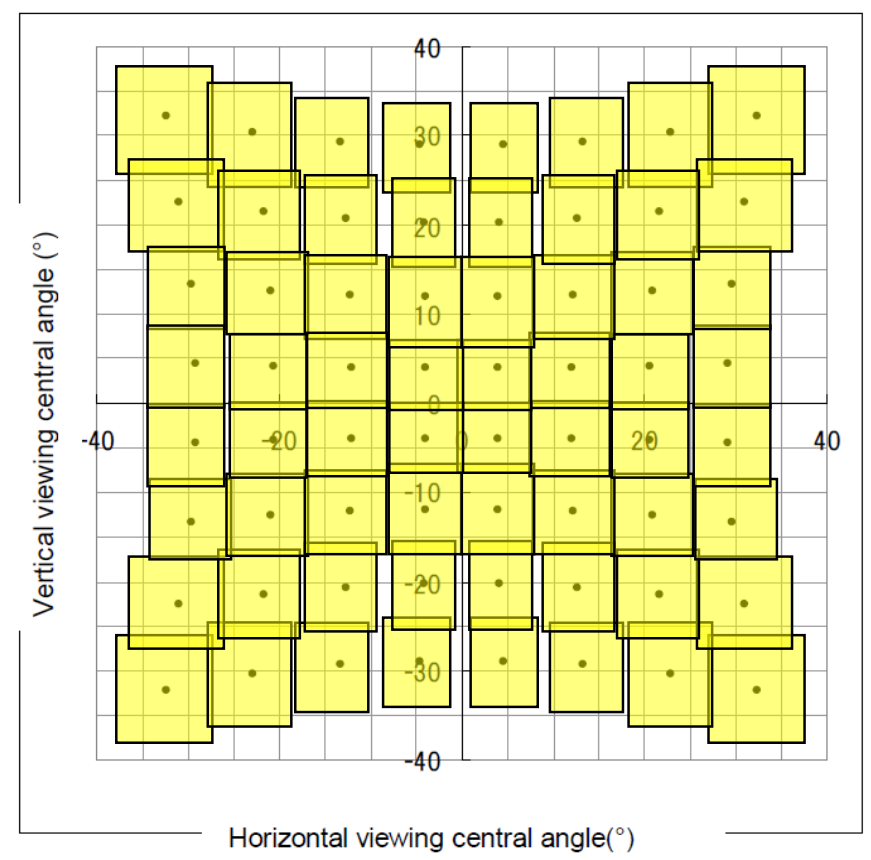
\includegraphics[width=0.6\textwidth]{figures/grideye_detectionarea.PNG}
  \caption{Detection area of each pixels of the Grideye sensor}\label{fig:grideyedetectionarea}
\end{figure}
\begin{equation}\label{eq:brownscorrection}
  r_c = r_u + K_1r_u^3+K_2r_u^5
\end{equation}
\section{Temperature Sensor}
The AMG8833 comes along with a on-board thermistor which measures its working temperature. \citeauthor{trofimova2017indoor} \cite{trofimova2017indoor} estimate the ambient temperature with the thermistor reading because they have a linear dependence. Nevertheless, an external temperature sensor that reads the accurate room temperature is useful, especially in case the IR module malfunctions.

We have chosen a DHT11 temperature and humidity sensor \cite{dht11} for this purpose. It measures the surrounding temperature at $1^\circ C$ precision.
\section{Main Processor}
The microprocessor should have one I2C interface to retrieve data from the IR camera. Since a new frame must be read every 0.1 second otherwise it will be covered by following frames, a realtime task support is required. The MCU should have a on-board radio component to send out data without an edge device. Besides, for debug purpose we want to store the frame sequences and let the tracker replay them frame by frame, an UART interface is required to simulate the camera frame input.

Our choice for the main processor is a ESP32-WROVER module from Espressif \cite{esp32wroverboard}. The specifications are shown in \autoref{tab:esp32wrover}.

The ESP32 board contains not merely a microprocessor, but also a set of out-of-box development firmware such as Wifi and bluetooth protocol, see \autoref{fig:ESP32diagram}. The board could be run as bare metal, however, the ESP-IDF (Espressif Internet-of-things Development Framework) empowers it to run on a adapted version of FreeRTOS \cite{esp32freertos}. In a RTOS (real-time operating system), each logically independent code snippet could be encapsulated as a task. The RTOS task scheduler divides CPU process time to tiny time slices (1 millisecond), and always assign a time slice to the task with the highest priority in the ready list at that moment. A task will be blocked if it requires a resource that is not available, and it will not participate in task scheduling until the required resource is available again. By this way, a strong realtime response performance is largely guaranteed, unless the processor's maximum computation power is exceeded.

The ESP32-WROVER module features a dual-core architecture. It contains two Xtensa CPU \cite{xtensa} with a frequency up to 240MHz. Wireless communication through Wifi or BLE is inherently handled by the first core, while user applications could be attached to either core. The powerful computational capacity yet a relative cost (€10) made it our first choice for the main processor.
\begin{table}
  \centering
\begin{tabular}{l|ll}
                & ESP32-WROVER     & Required \\ \hline
I2C interface   & 2                & 1        \\
UART interface  & 3                & 1        \\
GPIO pins       & \textgreater{}10 & 1        \\
realtime task   & FreeRTOS         & yes      \\
radio component & Wifi, bluetooth  & yes      \\
flash           & 4MB              & -        \\
RAM             & 520KB            & -
\end{tabular}
  \caption{Specifications of the ESP32-WROVER module}\label{tab:esp32wrover}
\end{table}
\begin{figure}
  \centering
  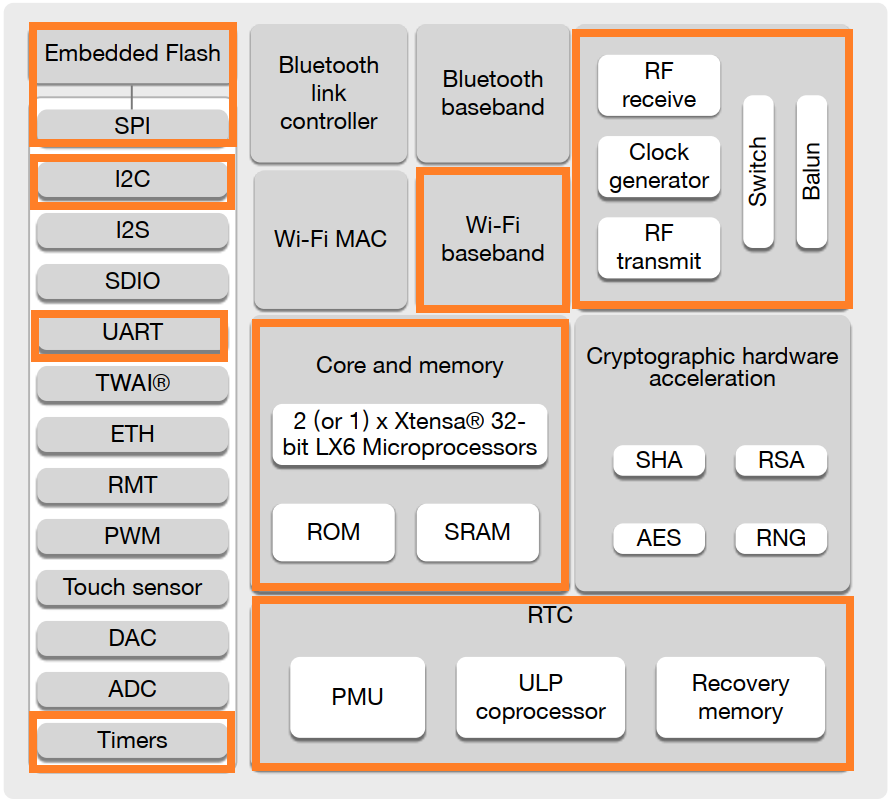
\includegraphics[width=0.8\textwidth]{figures/ESP32diagram.PNG}
  \caption{Functional block diagram of ESP32 chip}\label{fig:ESP32diagram}
\end{figure}


The total cost of our design is €35, including an AMG8833 Grideye (€20), an ESP32 board (€10) and a DHT11 temperature sensor (€5).

